% !TEX TS-program = xelatex

\chapter{Geometric models}
\label{chapt:4}

Julia |Plasm| is the best choice to write symbolic geometric models for Building Information Modeling (BIM) and Computer-Aided Design (CAD).  Geometric models specify the physical appearance of Architecture, Engineering, and Construction products at any scale, from structural and envelope components to whole buildings and built environments, and are used for design, tender, contract, and collaboration. We ported the  functional language |Plasm| to Julia for better supporting design, model generation, and visualization of geometric objects.
In this chapter we introduce the great expressive power of |Plasm| geometric types and parametric functions, as well the simple methods used to build parametric assemblies, where objects itself can be used as actual parameters. We show also that |Plasm| offers a  general mechanism (Julia dictionaries) to export models characterized by colors, textures, materials, and so on. |Plasm| can be even embedded in the |Jupiter| platform in order to document the design choices step-by-step in digital notebooks.

\section{Plasm geometric types}\label{sect:4-1}

Even if Julia does not pretend the user specifies the type of data objects, which are inferred at compile time, it may always be useful to annotate with their type the parameters and the returned value from function applications in order to get faster codes from the Julia compiler. The best reason concerns program documentation, making it easier to understand the Julia's sources.

Let's remember that |Plasm| derives from three founts: (1) the classic |PLaSM| set up on |FL| functional combinators; (2) the porting to Python (object-oriented language), and finally (3) the embedding into Julia (functional and multi-paradigm), after ten years of algebraic research finalized to understand the role of topology in elaborating digital  geometric models. 

This development defined different data types and user structures, which the current version of the language proudly unifies by scheduling them to different roles and uses.
 

\begin{enumerate}
\item 
The Hierarchical Polyhedral Complex, now denoted in Julia |Plasm| as the |Hpc| datatype, was characterized by models defined as aggregation of multidimensional convex cells, described only by their vertices and by multidimensional affine matrices.

\item 
Our research about algebraic topology of geometric design directed us to design the Linear Algebraic Representation, currently the |Lar| datatype, used to work with chain complexes, and able to  fully specify the geometry and topology of the \emph{solid objects} under consideration.

\item 
Finally, a third Julia user-defined |struct|, named |Geo| for Geometry, is being used as container of huge datasets for |Plasm|-coded applications of |BIM| objects and 3D point clouds from surveys.  
\end{enumerate}


\subsection*{Hpc Type}\label{sect:4-1-1}

This recursive type is mainly used for geometric object definition, including the hierarchical values generated by the |STRUCT| function, and interactive graphics visualization on the display device.

An object of |Hpc| type has three fields: a multidimensional matrix |T::MatrixNd|; a vector |childs| (i.e., children) either of elements |Hpc| or of elements |Geometry|, and a |Properties| field of dictionary type, i.e., |Dict{Any, Any}|.

The |mutable struct Hpc| is a typical recursive data structure to represent dynamically a data object of tree type, where the | children | nodes of a node may be in any number since stored into a Julia’s |Vector|.

\begin{lstlisting}[language=JuliaLocal, style=julia, mathescape = true] 
mutable struct Hpc
T::MatrixNd
childs::Union{Vector{Hpc}, Vector{Geometry}}
properties::Dict{Any, Any}
# constructor
   function Hpc(T::MatrixNd=MatrixNd(0), childs:: Union{Vector{Hpc}, Vector{Geometry}}=[], properties=Dict())
      self = new()
      self.childs = childs
      self.properties = properties
      if length(childs) > 0
         Tdim = maximum([dim(child) for child in childs]) + 1
         self.T = embed(T, Tdim)
      else
         self.T = T
      end
      return self
   end
end
\end{lstlisting}



\subsection*{Lar Type}\label{sect:4-1-2}

The |mutable struct Lar| is used to represent synthetically a generic cellular or chain complex, together with some of its properties. Given |obj::Lar|, it represents with |obj.d|, |obj.m|, |obj.n|, |obj.V|, and |obj.C|, respectively, the intrinsic dimension (1 for curves, 2 for surfaces, 3 for solids), the number of its coordinates, the number of vertices, and a dictionary of of chain bases or chain operators, stored when already available throughout a computation.

\begin{lstlisting}[language=JuliaLocal, style=julia, mathescape = true] 
mutable struct Lar
   d::Int # intrinsic dimension
   m::Int # embedding dimension (rows of V)
   n::Int # number of vertices  (columns of V)
   V::Matrix{Float64} # object geometry
   C::Dict{Symbol, AbstractArray} # object topology (C for cells) 
   # inner constructors
   Lar() = new( -1, 0, 0, Matrix{Float64}(undef,0,0), Dict{Symbol, AbstractArray}() )
   Lar(m::Int,n::Int) = new( m,m,n, Matrix(undef,m,n), Dict{Symbol,AbstractArray}() )
   Lar(d::Int,m::Int,n::Int) = new( d,m,n, Matrix(undef,m,n), Dict{Symbol,AbstractArray}() ) 
   Lar(V::Matrix) = begin m, n = size(V); new( m,m,n, V, Dict{Symbol,AbstractArray}() ) end
   Lar(V::Matrix,C::Dict) = begin m,n = size(V); new( m,m,n, V, C )  end
   Lar(d::Int,V::Matrix,C::Dict) = begin m,n = size(V); new( d,m,n, V, C )  end
   Lar(d,m,n, V,C) = new( d,m,n, V,C )
end
\end{lstlisting}



\subsection*{Geo type}\label{sect:4-1-3}

A |mutable struct Geometry| is used as a container for single whole geometric objects, allowing to store the various dimensional cellular subcomplexes that partition the geometric value. Conversely, any hierarchical assembly is stored in |Plasm| within a mixture of |Hpc| and |Geometry| nodes. The |Geometry| data structure contains arrays of integers, denoting the ordered bases of the topological chains of different dimensions that decompose the represented geometric value. It also contains a numeric |db| (data base), implemented as a Julia dictionary with key the (suitably rounded) coordinate vector sof vertex |point| and with value the corresponding integer index.

\begin{lstlisting}[language=JuliaLocal, style=julia, mathescape = true] 
mutable struct Geometry
   db::Dict{Vector{Float64}, Int}
   points::Vector{Vector{Float64}}
   edges::Vector{Vector{Int}}
   faces::Vector{Vector{Int}}
   hulls::Vector{Vector{Int}}
   # constructor
   function Geometry()
   self = new(
      Dict{Vector{Float64}, Int}(),
      Vector{Vector{Float64}}(),
      Vector{Vector{Int}}(),
      Vector{Vector{Int}}(),
      Vector{Vector{Int}}(),
   )
   return self
   end
end
\end{lstlisting}


\subsection*{Topological types}\label{sect:4-1-4}

Some abstract types are defined in |Plasm| in order to characterize and document the type of variables and/or parameters within complicated definitions and function codes. They are mainly used within the structures of |Lar| type, to document the topology, and are defined as global |const| symbols.

\begin{lstlisting}[language=JuliaLocal, style=julia, mathescape = true] 
const Points = Matrix{number}
const Cells = Vector{Vector{Int}}
const Cell = SparseVector{Int8, Int}
const Chain = SparseVector{Int8,Int}
const ChainOp = SparseMatrixCSC{Int8,Int}
const ChainComplex = Vector{ChainOp}
\end{lstlisting}

The |Cells| type stores the cellular bases and some subsets of cells as |Vector| of |Vector| of integers. The |Cell| type is utilized to memorize a single cell's (sparse)  representation. The |Chain| type item equals the cell type, and is used only for documentation aims. The |ChainOp| type allows the storage of the topological operators, including boundary and coboundary, and other higher degree operators, e.g., |FV|. The |ChainComplex| type is employed as the multidimensional |Vector| store of chain complexes, by now only in 2D and 3D, with two and three |ChainOp| sparse matrices, respectively.

\begin{coding}[3-cube topology is a ChainOp object]\
Whereas the expression |cube.C[:FV]| returns a dictionary value of type |Cells|, which contains the basis of our cubic cellular complex, |top| is of |ChainOp| type:

\begin{lstlisting}[language=JuliaLocal, style=julia, mathescape = true] 
cube = LAR(CUBE(3))			#=
Lar(3, 3, 8, [3.0 0.0 … 3.0 0.0; 3.0 3.0 … 3.0 3.0; 0.0 0.0 … 3.0 3.0], Dict{Symbol, AbstractArray}(:CV => [[1, 2, 3, 4, 5, 6, 7, 8]], :FV => [[1, 2, 3, 4], [3, 4, 5, 6], [1, 3, 5, 7], [2, 4, 6, 8], [1, 2, 7, 8], [5, 6, 7, 8]], :EV => [[3, 4], [2, 4], [1, 2], [1, 3], [5, 6], [4, 6], [3, 5], [5, 7], [1, 7], [6, 8], [2, 8], [7, 8]])) =#

FV = cube.C[:FV]			#=
6-element Vector{Vector{Int64}}:
 [1, 2, 3, 4]
 [3, 4, 5, 6]
 [1, 3, 5, 7]
 [2, 4, 6, 8]
 [1, 2, 7, 8]
 [5, 6, 7, 8]

KFV = lar2cop(FV)			#=
6×8 SparseArrays.SparseMatrixCSC{Int8, Int64} with 24 stored entries:
 1  1  1  1  ⋅  ⋅  ⋅  ⋅
 ⋅  ⋅  1  1  1  1  ⋅  ⋅
 1  ⋅  1  ⋅  1  ⋅  1  ⋅
 ⋅  1  ⋅  1  ⋅  1  ⋅  1
 1  1  ⋅  ⋅  ⋅  ⋅  1  1
 ⋅  ⋅  ⋅  ⋅  1  1  1  1			=#
\end{lstlisting}
Of course, |(typeof(FV)==Cells) && (typeof(KFV)==ChainOp) # => true|.
\end{coding}

\begin{remark}[About sparsity]
While in this small case, the |FV| matrix is not very sparse in this small case, the sparsity overgrows as the cellular complex proliferates since the non-zero elements grow linearly with the number of cells. In contrast, the zero elements grow quadratically (with the matrix elements).
\end{remark}


\section{Plasm parametric primitives}\label{sect:4-2}

In this section, we introduce and exemplify several features of the working of |Plasm| with geometric objects. This system is quite different from most geometric and graphics systems since it is based on |FL|-style combinators.


\subsection{Geometric Transformations in Julia Plasm}\label{sect:4-2-1}

The user interface to affine coordinate transformation of geometric objects is given through standard Julia functions and matrices. Internally, |Plasm| implements such mapping of local coordinates using its own multidimensional matrix type, called |MatrixNd|, and the use of the field |T::MatrixNd| within the recursive datatype |Hpc|.

\begin{definition}[Geometric transformation]
A \emph{geometric transformation} is a bijective function, i.e., a one-to-one (injective) and onto (surjective) mapping $\mathbb{E}^d \to \mathbb{E}^d$. 
\end{definition}

By definition, geometric transformations of plane or space are invertible, and so represented by invertible square matrices. We will see that \emph{rotation}, \emph{scaling}, and \emph{shearing} are linear transformations; \emph{translation} is affine. 


\subsubsection*{Homogeneous Coordinates}

In computer graphics the \emph{homogeneous coordinates} are often used instead of Cartesian coordinates. In the homogeneous plane or space, lines are mapped to lines, but parallel lines are not conserved parallel. The main reason for this change is the ability to treat affine maps (translation) as linear, and combine smoothly with linear maps (rotation, scaling, etc.)

In homogeneous coordinates the Euclidean plane $\mathbb{E}^2 \,\backslash\, \{\v{0}\}$ is considered in bijective correspondence with the bundle of lines in $\mathbb{E}^3 \,\backslash\, \mathbb{E}^2$ (a model for the projective plane) so that each point $(x,y)\in\E^2$ corresponds to a line $\lambda(W, X, Y)$ such that $(x, y) \equiv \frac{W}{W}, \frac{X}{W}, \frac{Y}{W}) = (1, x, y)$. Same for each $\E^d$, $d \geq 2$. After the division, homogeneous coordinates are said \emph{normalized}.

\begin{figure}[htbp] %  figure placement: here, top, bottom, or page
   \sidecaption[t]
   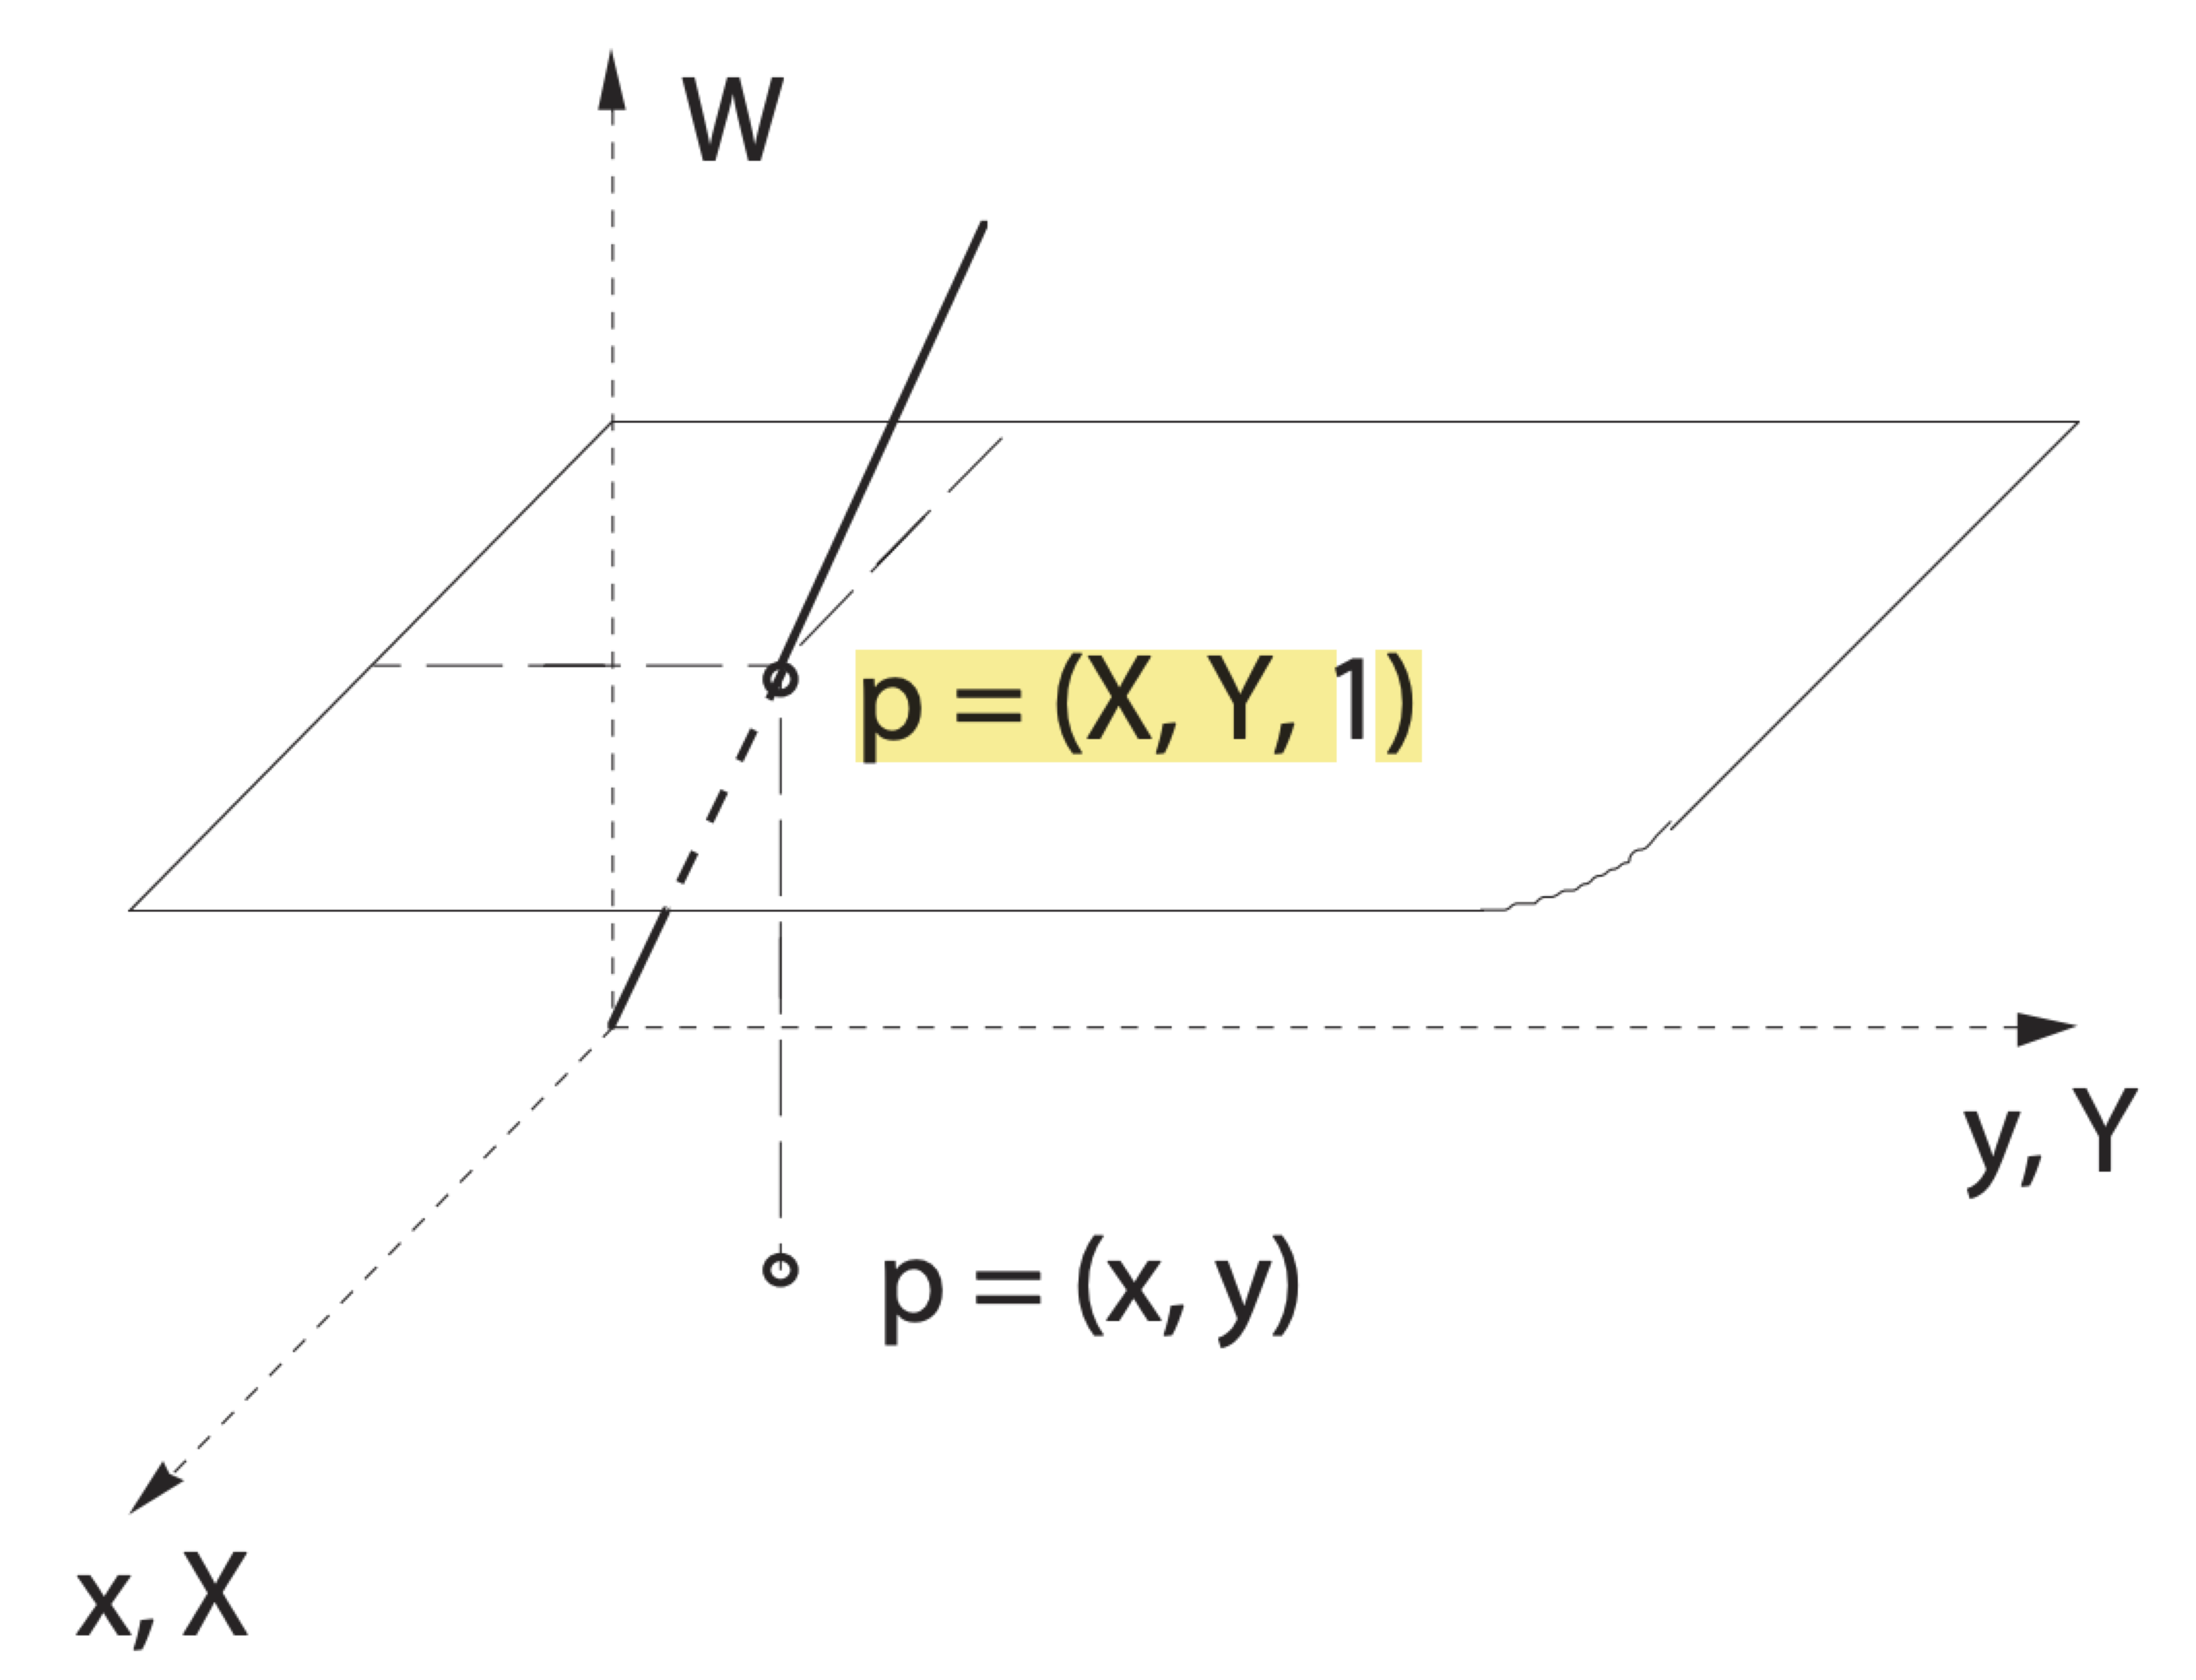
\includegraphics[width=2in]{chapter-04/figs/homog-2d} 
   \caption{The homogeneous plane is a model of a projective plane, where all finite points have a homogeneous coordinate equal to one, and the points at infinity have it equal to zero. All the points at infinity form the line at infinity, and all the lines at infinity form the plane at infinity.}
   \label{fig:example}
\end{figure}

In |Plasm|, by design choice to make the multidimensional approach to geometric design more accessible, the added homogeneous coordinate is the first, not the last, as we may see in many computer graphics books.

Even more, for the sake of clarity we can use the |HOMO| operator to transform a $d\times d$ matrix in a $(d+1)\times(d+1)$ matrix, i.e., a $3\times 3$ on the 2D plane and $4\times 4$ on 3D space. The type of returned matrix is |MatrixNd|, which is used for dimension-independent programming.

Homogeneous coordinates allow to combine linearly all transformations, using products of their matrices in homogeneous coordinates. In the remainder of this section we describe the geometric effect of each transformation and the structure of the corresponding matrices. 

\begin{remark}The reader should note that our maps or transformations are invertible functions of a space into itself (automorphisms), represented (even translation, as we will see) by square matrices, i.e. are \emph{rank 2} tensors. Since they are also |Plasm| functions, can be \emph{applied} to geometric objects; as matrices, they multiply the object coordinates.
\end{remark}




\subsection*{2D rotation}\label{sect:4-2-1}

In a \emph{planar rotation} all points of the 2D plane move along an arc of circle, with same angle at center, while the center is the only fixed point. In  a \emph{space rotation} there is a straight line of fixed points (the axis) passing for the origin. All the other 3D points describe a circle arc with the same angle along the plane (orthogonal to rotation axis) which they belong to. 

Let us show (see Figure~\ref{fig:rotmatrix}) how unit vectors $\v{e}_1 = \vet{1 \\ 0}$ and $\v{e}_2 = \vet{0 \\ 1}$, columns of the matrix $\mat{\v{e}_1 & \v{e}_2 } $ are transformed by the (yet unknown) $\T{R}(\alpha)$ rotation matrix into the columns of the matrix at right-hand side:
\[
\mat{\cos\alpha & -\sin\alpha\\ \sin\alpha & \cos\alpha}
=
\T{R}(\alpha)\,\mat{\v{e}_1 & \v{e}_2 }. 
\quad
\mbox{Hence we have:}
\quad
\T{R}(\alpha) = \mat{\cos\alpha & -\sin\alpha\\ \sin\alpha & \cos\alpha}
\]


There is only one class of planar rotations, parameterized by $\alpha$, the \emph{rotation angle} about the origin. Conversely, we will see three classes of elementary space rotations, parameterized by $\alpha_x, \alpha_y, \alpha_z$, the rotation angles about each coordinate axis.


\begin{coding}[Plasm notation for rotation]
The plane rotation function in |Plasm| is: |R([1,2])($\alpha$)| because its effect is to change the first and second coordinates of the 2D model it is applied to. They are applied to a planar geometric object of |Hpc| type, by using the |STRUCT| operator (see Section~\ref{}) that contains |Hpc| values and transformation tensors:
\begin{lstlisting}[language=JuliaLocal, style=julia, mathescape=false]
SQUARE(d) = CUBOID([d,d])		#=
SQUARE (generic function with 1 method)		=#

obj = R(1,2)(π/4)(SQUARE(1))		#=
Hpc(MatrixNd([[1.0, 0.0, 0.0], [0.0, 0.7071067811865476, -0.7071067811865475], [0.0, 0.7071067811865475, 0.7071067811865476]]), Hpc(MatrixNd(3), Hpc(MatrixNd(3), Geometry([[0.0, 0.0], [1.0, 0.0], [1.0, 1.0], [0.0, 1.0]], hulls=[[1, 2, 3, 4]])))) =#

VIEW(obj)
\end{lstlisting}
\end{coding}

\begin{remark}
|CUBOID(shape)::Hpc| is the generator of multidimensional hyper-par\-allelo\-pipeds, depending on length and content of |shape| vector. 

|CUBOID([1,1])| is the unit square;  |CUBOID([1,2,3])| is the parallelopiped of sides 1, 2, and 3; 
|CUBOID([1,1,1,1])| is the 4D unit hypercube.
\end{remark}


\subsection*{Elementary rotations}

The multidimensional |Plasm| language has the following definition of elementary rotation, that allows to rotate a $r$-model ($r\leq d$) in any dimension $d\geq 2$.

\begin{definition}[Elementary rotation]
The reader should note that the \emph{elementary} rotation is defined in any dimension $d$  such that only $2$ coordinates are changed by the rotation.
\end{definition}

\begin{remark}
It is easy to see that in any dimension $d$ there are |binomial$(d,2)$| elementary rotations, how many are the ways to choose $2$ coordinates over $d$. Hence we have $1$ for $d=2$, 3 for $d=3$, 6 for $d=3$, and so on.
\end{remark}


Assume that the rotation axes are $\v{e}_1, \v{e}_2, \v{e}_3$, with rotation angles $\alpha, \beta, \gamma$ respectively. The corresponding elementary matrices, derivable as before by change of coordinates, are:
\begin{equation}\footnotesize
\T{R}_x(\alpha) = \mat{1 & 0 & 0 \\ 0 & \cos\alpha\ &  -\sin\alpha\\ 0 & \sin\alpha & \cos\alpha},\ 
\T{R}_y(\beta) = \mat{\cos\beta & 0 & \sin\beta\\ 0 & 1 & 0 \\ -\sin\beta\  &  0 & \cos\beta},\ 
\T{R}_z(\gamma) = \mat{\cos\gamma & -\sin\gamma & 0\\ \sin\gamma & \cos\gamma & 0\\ 0 & 0  &1}
\end{equation}

In |Plasm| the elementary rotations are represented, respectively, by the tensors: |R([2,3])($\alpha$)|, |R([1,3])($\beta$)|, and |R([1,2])($\gamma$)|. 
\begin{coding}[Elementary rotation] We use an interesting 3D polyhedron, called permutahedron, to show the application of the tensor |R([1,2])(pi/2)| to it:
\begin{lstlisting}[language=JuliaLocal, style=julia, mathescape=false]
obj = R([1,2])(pi/2)( PERMUTAHEDRON(3) );
VIEW( obj )
\end{lstlisting}
\end{coding}

\begin{remark}[Reduction of visual noice]
Just note that in all |Plasm| geometric operators, the constraint of using functions as unary has been relaxed, in order to make possible to write, e.g., |obj = R(1,2)(pi/2)(obj)| instead than |obj = R([1,2])(pi/2)(obj)|. In the remainder we use always this new style.
\end{remark}


\begin{coding}[Permutahedron] The reader might be curious to see how such important and beautiful polyhedron~\cite{wiki:pao:100} whose vertex coordinates are the permutations of the first $d$ natural numbers. Iy is generated in |Plasm|:
\begin{lstlisting}[language=JuliaLocal, style=julia, mathescape=false]
function PERMUTAHEDRON(d)
	vertices = ToFloat64(PERMUTATIONS(collect(1:d+1)))
	center = MEANPOINT(vertices)
	cells = [collect(1:length(vertices))]
	object = MKPOL(vertices, cells, [[1]])
	object = T(INTSTO(d))(-center)(object)
	for i in 1:d
		object = R(i,d+1)(pi/4)(object)
	end
	object = PROJECT(1)(object)
	return object
end
\end{lstlisting}
The |Plasm| function |INTSTO($d$)| (integers to $d$) is used to generate the sequence |[1,2,$\ldots$,d]|, extremes included. The other functions are easy to understand.
\end{coding}




\subsection*{General rotation in 3D}

A rotation of 3D space has a fixed line of points (the rotation axis) passing through the origin. We may compute the corresponding matrix as a function of a direction vector for the axis and a real value for the rotation angle. For this purpose we can compone three linear transformations by multiplication of their matrices.  Therefore we have:

\begin{definition}[General 3D rotation with axis $d$ and angle $\alpha$]
Clearly, the ordering of transformations is from right to left:
\[
\T{R}(\v{d},\alpha) = \T{Q}^{-1}(\v{d})\, \T{R}_z(\alpha)\, \T{Q}(\v{d})
\]
First, a space rotation that brings the vector $d$ on a coordinate axis, say $\v{e}_3$; second, a space rotation $\T{R}_z(\alpha)$ about the $z$-axis; third, the inverse of the first transformation, so to bring the rotation axis in its original direction.
\end{definition}

$\T{Q}(\v{d})$ must transform the unit vector $\v{d}$ to the $\v{e}_3$ unit vector. So, we may compute the coordinate transformation that brings three orthonormal vectors $(\v{u}_1, \v{u}_2, \v{u}_3)$ to become the standard basis $(\v{e}_1, \v{e}_2, \v{e}_3)$. We can choose the triple:
\begin{eqnarray}
\v{u}_3 &=& \v{d}/\,\|\v{d}\|,\nonumber\\
\v{u}_2 &=& (\v{u}_3 \times \v{e}_3)/\,\|\v{u}_3 \times \v{e}_3\|,\\
\v{u}_1 &=& \v{u}_2 \times \v{u}_3,\nonumber
\end{eqnarray}
to write the transformation of coordinates:
\[
(\v{e}_1, \v{e}_2, \v{e}_3) = \T{Q}(\v{d})\, (\v{u}_1, \v{u}_2, \v{u}_3)
\]
so that we have:
\[
\T{Q}(\v{d}) = (\v{u}_1, \v{u}_2, \v{u}_3)^{-1}
\]
But $\T{Q}(\v{d})$ maps orthonormal vectors to orthonormal vectors, hence it is a normal
transformation, so its inverse is equal to its transpose. So, we can write:
\begin{equation}
\T{R}(\v{d},\alpha) = \T{Q}^{t}(\v{d})\, \T{R}_z(\alpha)\, \T{Q}(\v{d}).
\end{equation}


\begin{coding}[3D General Rotation matrix]
Let’s use a test-driven programming style, with parameter values easy to test
Rotate of 45 degrees about the diagonal axis the unit cube with a vertex on the origin, i.e. the model generated by the |CUBE(1)| expression in |Plasm|. 
We may follow this procedure using a functional approach:

\begin{lstlisting}[language=JuliaLocal, style=julia, mathescape=false]
using Plasm, LinearAlgebra
d = [1,1,1];
u₃ = normalize(d);
u₂ = normalize(u₃ × [0,0,1]);
u₁ = u₂ × u₃;
\end{lstlisting}
and write the following matrix for the transformation of coordinates that maps the $\v{e}_3$ axis to the direction of the |d| vector. 
\begin{lstlisting}[language=JuliaLocal, style=julia, mathescape=false]
Q(d) = [u₁ u₂ u₃]'
\end{lstlisting}
The single quote stands for the Julia |transpose| of a matrix.
\end{coding}


\begin{figure}[htbp] %  figure placement: here, top, bottom, or page
\begin{minipage}[c]{0.35\textwidth}
   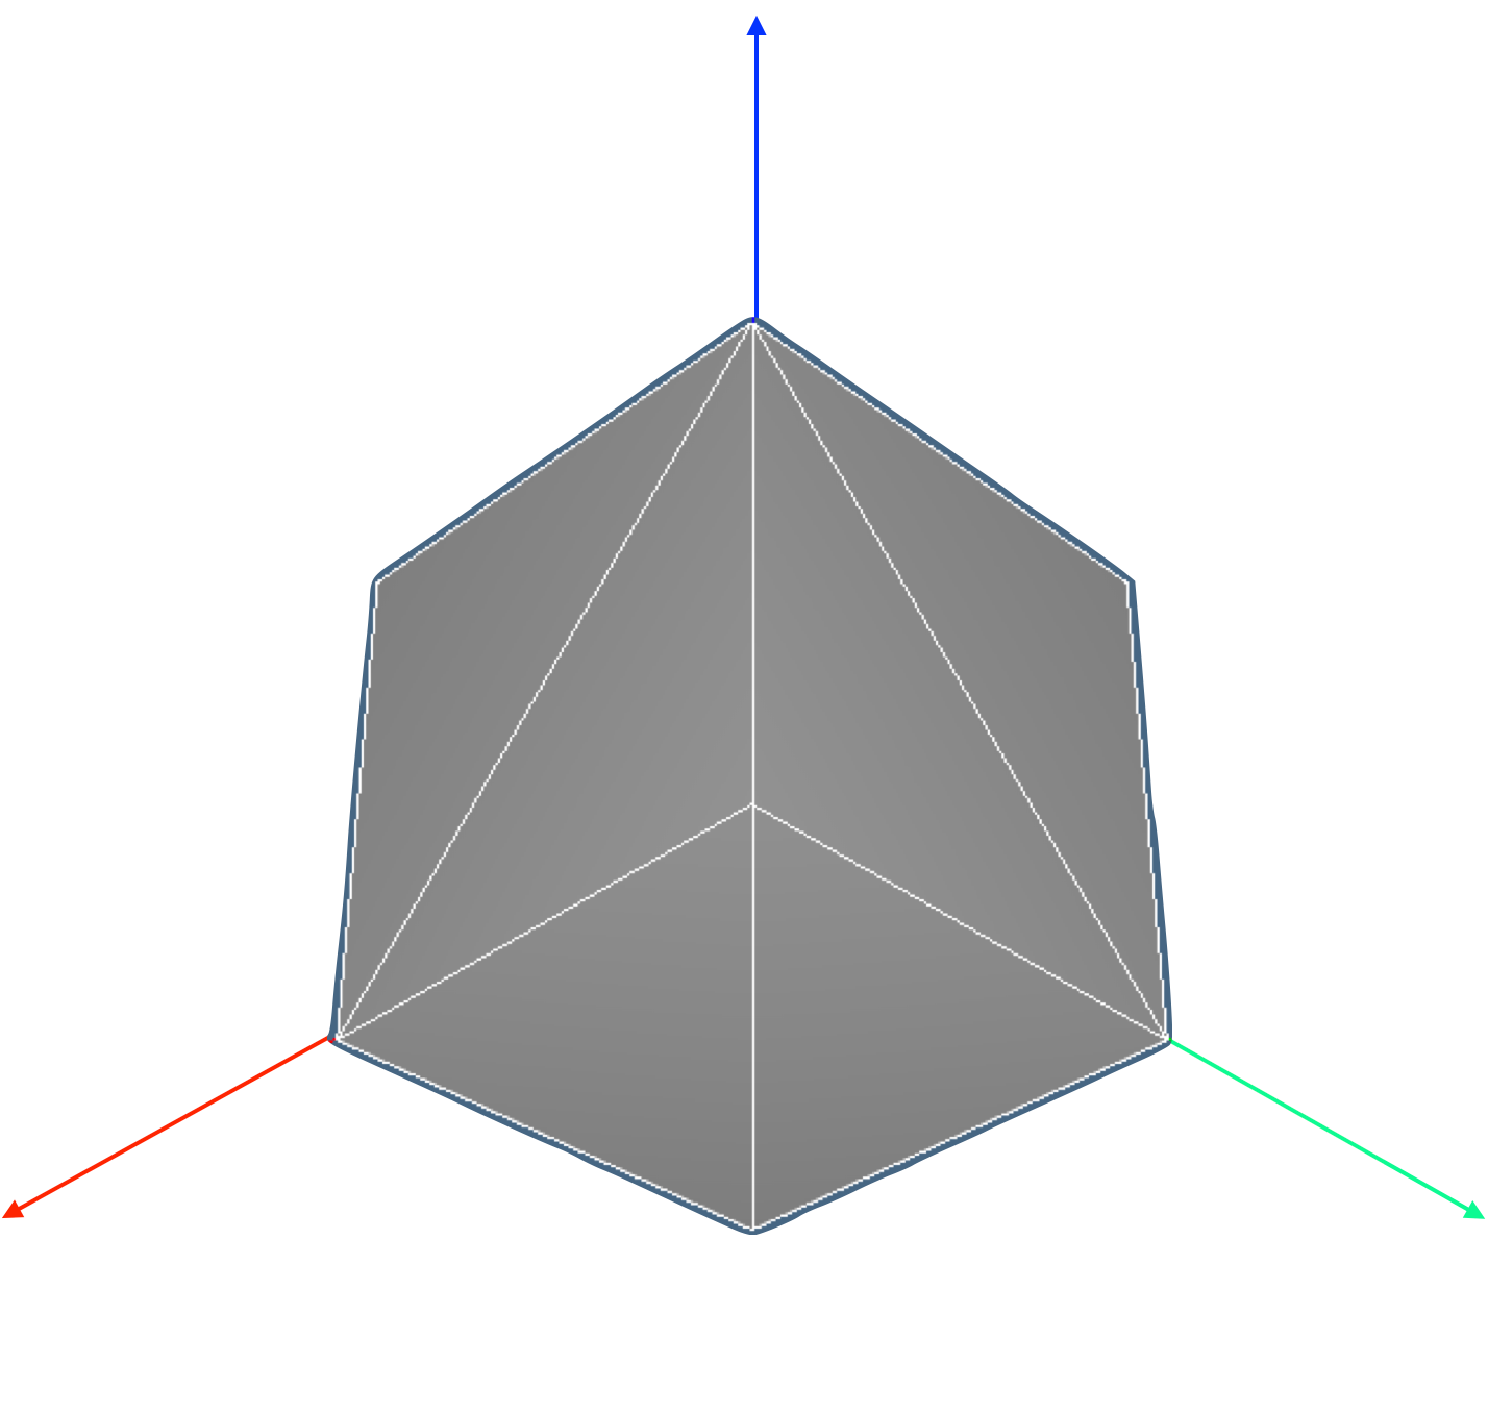
\includegraphics[width=2in]{chapter-04/figs/GRcube} 
\end{minipage}
\hfill
\begin{minipage}[c]{0.55\textwidth}
\begin{lstlisting}[language=JuliaLocal, style=julia, mathescape=false]
rotated = GR([1,1,1],π/3)(CUBE(1))
VIEW(rotated)
\end{lstlisting}
\end{minipage}
\end{figure}


\begin{coding}[General 3D rotation tensor]
In what follows, |MAT| transforms a Julia |Matrix| into a |Plasm| tensor applicable to |Hpc| values. 
The |HOMO| function apply to  a square matrix, adding new unitary first row and column, for homogeneous coordinates (see Section~\ref{}).  
\begin{lstlisting}[language=JuliaLocal, style=julia, mathescape=true]
GR(d,α) = MAT(HOMO(Q(d)')) ∘ R(1,2)(α) ∘ MAT(HOMO(Q(d)))
\end{lstlisting}
The |GR| (general rotation) is a |Plasm| tensor depending on the axis |d| and the angle |$\alpha$|. 
Our geometric model is therefore rotated and viewed as follows.
\end{coding}



\subsection*{Scaling}\label{sect:4-2-2}

In a scaling transformation, all points are moved along the line passing for the origin they belong to.  The scaling is said \emph{elementary} when only one of the coordinates changes. There are two scaling parameters $s_x, s_y$ in 2D geometry and three scaling parameters $s_x, s_y, s_z$ in 3D, to be used in scalar products by the point coordinates.
The transformation can be a \emph{dilatation} of space when scaling parameters are greter than one, or a \emph{contraction} of space when scaling parameters are lesser than one.
\[
S(s_x,s_y,s_z) = \mat{s_x & 0 & 0\\ 0 & s_y & 0\\ 0 & 0 & s_z},\ 
S_x = \mat{s_x & 0 & 0\\ 0 & 1 & 0\\ 0 & 0 & 1},\ 
S_y = \mat{1 & 0 & 0\\ 0 & s_y & 0\\ 0 & 0 & 1},\ 
S_z = \mat{1 & 0 & 0\\ 0 & 1 & 0\\ 0 & 0 & s_z} 
\]
The scaling matrices are diagonal.
The origin remains fixed. In fact: \[S\,\vet{0 &0 & 0}^t = \vet{0 & 0 & 0}^t.\] 
Hence, a scaling transformation is linear. It is easy to see that  scale transformations are multiplicative, commutative, and associative because the matrix is diagonal:
\[
\T{S}(s_x, s_y, s_z) = \T{S}_x(s_x)\, \T{S}_y(s_y)\, \T{S}_z(s_z)$.
\]
\begin{coding}[How to scale a Plasm model?]
As in the previous coding example, let’s go to use the |cube(1)| as our model object.

\begin{lstlisting}[language=JuliaLocal, style=julia, mathescape=false]
scaledcube1 = S(1,2,3)(.1,.1,10)(CUBE(1))
scaledcube2 = S(3)(100)(CUBE(1))
\end{lstlisting}
\end{coding}


\begin{coding}[How to scale a Plasm model?]
Note that the effect of transformations impacts only the homogeneous matrices ahead of |Hpc| values. 
\begin{lstlisting}[language=JuliaLocal, style=julia, mathescape=false]
scaledcube1 = S(1,2,3)(.1,.1,10)(CUBE(1)) 	#=
Hpc(MatrixNd([[1.0, 0.0, 0.0, 0.0], [0.0, 0.1, 0.0, 0.0], [0.0, 0.0, 0.1, 0.0], [0.0, 0.0, 0.0, 10.0]]), Hpc(MatrixNd(4), Hpc(MatrixNd(4), Geometry([[0.0, 0.0, 0.0], [1.0, 0.0, 0.0], [0.0, 1.0, 0.0], [1.0, 1.0, 0.0], [0.0, 0.0, 1.0], [1.0, 0.0, 1.0], [0.0, 1.0, 1.0], [1.0, 1.0, 1.0]], hulls=[[1, 2, 3, 4, 5, 6, 7, 8]])))) =#
scaledcube2 = S(2)(100)(SQUARE(1)) 	#=
Hpc(MatrixNd([[1.0, 0.0, 0.0], [0.0, 1.0, 0.0], [0.0, 0.0, 100.0]]), Hpc(MatrixNd(3), Hpc(MatrixNd(3), Geometry([[0.0, 0.0], [1.0, 0.0], [1.0, 1.0], [0.0, 1.0]], hulls=[[1, 2, 3, 4]])))) =#
\end{lstlisting}
Of course, |S(1,2,3)(.1,.1,10)| and |S(2)(100)| are tensor objects.
\end{coding}


\begin{coding}[Construction of octahedron model]
As an exciting coding example, we show a simple construction of an octahedron model, starting from the 3D SIMPLEX model.
\begin{lstlisting}[language=JuliaLocal, style=julia, mathescape=false]
tetra = SIMPLEX(3);
twotetra = STRUCT( tetra, S(1)(-1), tetra );
fourtetra = STRUCT( twotetra, S(2)(-1), twotetra );
octahedron = STRUCT( fourtetra, S(3)(-1), fourtetra );
\end{lstlisting}

Looking at the whole cellular complex corresponding to the solid model |octahedron::Hpc| is worthwhile. For this purpose, we transform it into an object of |Lar| type:

\begin{figure}[htbp] %  figure placement: here, top, bottom, or page
\begin{minipage}[c]{0.35\textwidth}
   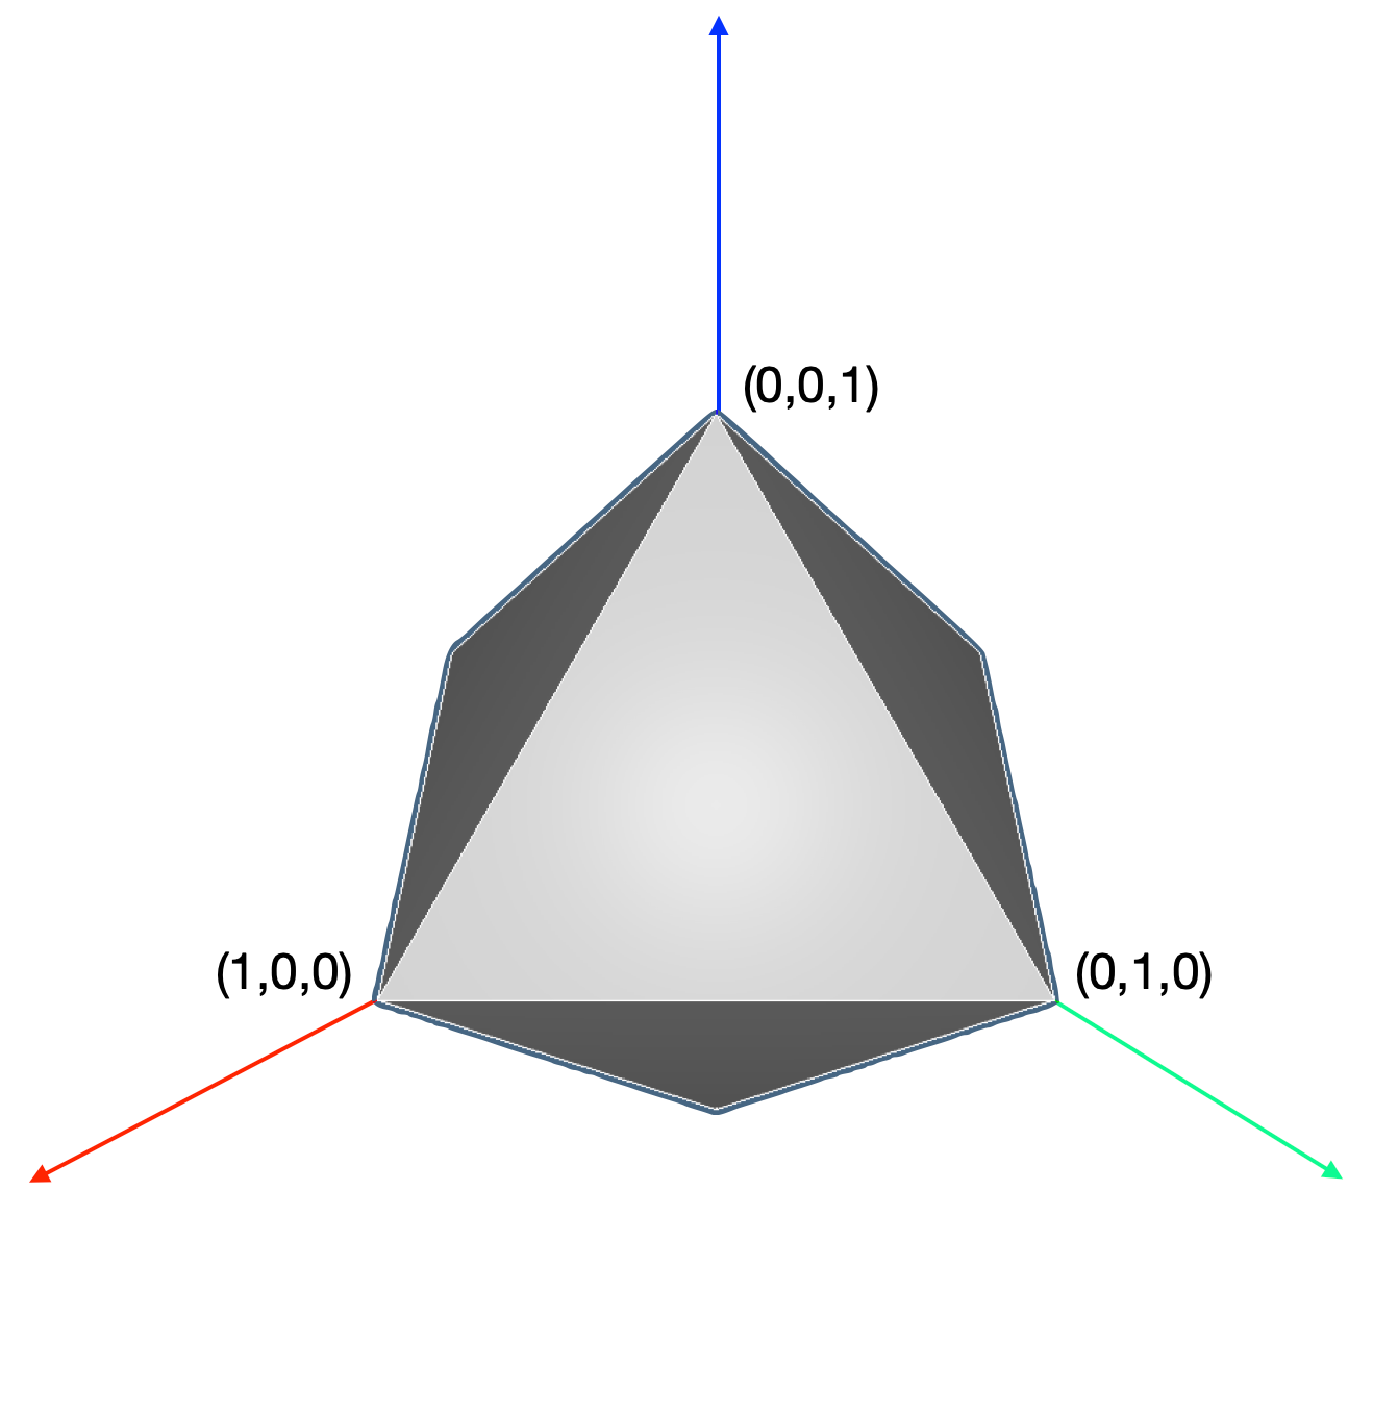
\includegraphics[width=\linewidth]{chapter-04/figs/octahedron} 
\end{minipage} \hfill
\begin{minipage}[c]{0.6\textwidth}
\begin{lstlisting}[language=JuliaLocal, style=julia, mathescape=false]
VIEW(octahedron::Hpc)
\end{lstlisting}
\caption{Plasm viewing generator expression. Remember that VIEW applies to Hpc values.}\label{fig:octahedron}
\end{minipage}
\end{figure}

\begin{coding}[The cellular complex]
Let’s note that the |octahedron::Hpc| is viewed, and that the |octahedron::Lar| is explored for stored data:\\
\begin{lstlisting}[language=JuliaLocal, style=julia, mathescape=false]
LAR(Octahedron).V 	#=
3×7 Matrix{Float64}:
  0.0  -1.0  0.0   0.0  1.0  0.0  0.0
 -1.0   0.0  0.0   0.0  0.0  1.0  0.0
  0.0   0.0  0.0  -1.0  0.0  0.0  1.0 	=#
LAR(Octahedron).C	#=
Dict{Symbol, AbstractArray} with 3 entries:
  :CV => [[1, 2, 3, 4], [1, 3, 4, 5], [2, 3, 4, 6], [3, 4, 5,…
  :FV => [[1, 2, 3], [2, 3, 4], [1, 3, 4], [1, 2, 4], [1, 3, …
  :EV => [[2, 3], [1, 3], [1, 2], [3, 4], [2, 4], [1, 4], [3,…=#
\end{lstlisting}

For |$\#$C, $\#$F, $\#$E, $\#$V|, we see, looking at |.V| and |.C| above:
\begin{lstlisting}[language=JuliaLocal, style=julia, mathescape=false]
AA(LEN)(values(Octahedron.C))'	#=
1×3 adjoint(::Vector{Int64}) with eltype Int64:
 8  20  18		=#
\end{lstlisting}
Therefore, we may see that the combinatorial (simplicial) complex corresponding to the 3D octahedron is made by 
8 + 20 + 18 + 7 = 53 cells of dimension 3, 2, 1, and 0, respectively (see Figure~\ref{fig:octahedron}).
\end{coding}




\section{Hierarchical assembly of geometric objects}\label{sect:4-3}


\section{Attach properties to geometry}\label{sect:4-4}


\section{Design documentation (Jupyter notebooks)}\label{sect:4-5}


\section{Export geometry}\label{sect:4-6}

